\documentclass{article}%
\usepackage[T1]{fontenc}%
\usepackage[utf8]{inputenc}%
\usepackage{lmodern}%
\usepackage{textcomp}%
\usepackage{lastpage}%
\usepackage{authblk}%
\usepackage{graphicx}%
%
\title{Characterization of a Large Outbreak by CTX{-}M{-}1{-}Producing Klebsiella pneumoniae and Mechanisms Leading to In Vivo Carbapenem Resistance Development}%
\author{Justin Ball}%
\affil{School of Pharmacy, Second Military Medical University, Shanghai, China}%
\date{01{-}01{-}2014}%
%
\begin{document}%
\normalsize%
\maketitle%
\section{Abstract}%
\label{sec:Abstract}%
In a News 8 investigation, we found human cells rapidly destroying fish in a lab test.\newline%
Now more than 1,000 patients {-}{-} and millions more around the world {-}{-} may benefit by seeing the results of our breakthrough on how RNAi, or natural messenger RNA, works.\newline%
When researchers gave cancer patients blood levels of the hormone angiotensin, they found low blood levels of the hormone made them go into remission.\newline%
Now, researchers at UC San Diego have another brain cancer treatment they believe will help if properly taken by patients.\newline%
The research from UC San Diego is on the verge of being published this month in the Journal of Oncology.\newline%
Some of the scientists said, We know that RNAi has several advantages over existing therapy, and we think we can improve the quality of patients lives and improve cancer death rates in that sense as well.\newline%
When asked about the possibility of using them to treat many types of cancer, one scientist added, Id have to make an effort to evaluate more patients.

%
\subsection{Image Analysis}%
\label{subsec:ImageAnalysis}%


\begin{figure}[h!]%
\centering%
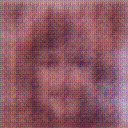
\includegraphics[width=150px]{500_fake_images/samples_5_331.png}%
\caption{A Close Up Of A Zebra In A Field}%
\end{figure}

%
\end{document}